
\section{Numerical Results}
\label{sec:results}
We first present convergence studies for both two- and three-dimensional test problems which illustrate the predicted convergence rates for the fully-discrete finite element method. We then apply our method to the popular 2D cantilever bracket problem and demonstrate that our stabilization techniques overcomes the spurious pressure oscillations that have been experienced by other methods. Finally, a 3D unconfined compression problem is presented that highlights the added mass effect of the method for different choices of the stabilization parameter $\delta$.

%\subsection{Implementation}
%For the implementation we used the C++ library libmesh \cite{kirk2007libmesh}, and the multi-frontal direct solver mumps \cite{amestoy2000multifrontal} to solve the resulting linear system.
%To solve the full Biot model problem (\ref{eqn:strong_cont_system_biot}), we need to solve the following linear system at each time step:
% \begin{equation*}
% \begin{bmatrix}
%  \mathbf{A} & 0 & \alpha\mathbf{B}^{T} \\
%  0 & \mathbf{M} & \mathbf{B}^{T} \\
% - \alpha \mathbf{B} & -\Delta t \mathbf{B} & c_{0}\mathbf{Q} +\mathbf{J}
% \end{bmatrix}
% \begin{bmatrix}
%  \mathbf{u}^{n} \\
%  \mathbf{z}^{n} \\
% \mathbf{p}^{n}
% \end{bmatrix}=
% \begin{bmatrix}
%  \mathbf{r} \\
%  \mathbf{s} \\
%  \Delta t \, \mathbf{g} - \mathbf{B} \mathbf{u}^{n-1} + c_{0}\mathbf{Q}\mathbf{p}^{n-1} + \mathbf{J} \mathbf{p}^{n-1}
% \end{bmatrix},
% \end{equation*}
% where we have defined the following matrices and vectors:
% \begin{eqnarray*}
%&&\mathbf{A}=[\mathbf{a}_{ij}], \;\; \mathbf{a}_{ij}=\int_{\Omega}2\mu_{s} \nabla \mathbf{\phi}_{i} : \nabla\mathbf{\phi}_{j} + \lambda (\nabla\cdot \mathbf{\phi}_{i}) (\nabla\cdot \mathbf{\phi}_{j}), \\
%&&\mathbf{M}=[\mathbf{m}_{ij}], \;\; \mathbf{m}_{ij}=\int_{\Omega}\permscalar  \mathbf{\phi}_{i} \cdot \mathbf{\phi}_{j}, \\
%&& \mathbf{B}=[\mathbf{b}_{ij}], \;\; \mathbf{b}_{ij}=-\int_{\Omega}  {\psi}_{i} \nabla \cdot \mathbf{\phi}_{j} , \\
%&&\mathbf{Q}=[\mathbf{q}_{ij}], \;\; \mathbf{q}_{ij}=\int_{\Omega}  {\psi}_{i} \cdot {\psi}_{j}, \\
%&&\mathbf{J}=[\mathbf{j}_{ij}], \;\; \mathbf{j}_{ij}=
% \delta \sum_{K} \int_{\partial k \backslash \partial \Omega} h_{\partial K} [{\psi}_{i}][{\psi}_{j}] \;\mbox{d}s, \\
%&&\mathbf{r}=[\mathbf{r}_{i}], \;\; \mathbf{r}_{i}=\int_{\Omega}  \mathbf{f}_{i} \cdot {\phi}_{i} + \int_{\Gamma_{t}}{\mathbf{t}_{N}}_{i} \cdot {\phi}_{i}, \\
%&&\mathbf{s}=[\mathbf{s}_{i}], \;\; \mathbf{s}_{i}=\int_{\Omega}  \mathbf{b}_{i} \cdot {\phi}_{i}-\int_{\Gamma_{p}} p_{D} {\phi}_{i} \cdot \mathbf{n}, \\
%&& \mathbf{g}=[\mathbf{g}_{i}], \;\; \mathbf{g}_{i}=\int_{\Omega}  g {\psi}_{i}.
% \end{eqnarray*}
%Here $\mathbf{\phi}_{i}$ are vector valued linear basis functions such that the displacement vector can be written as $\mathbf{u}^{n}= \sum_{i=1}^{n_{u}}\mathbf{u}^{n}_{i}\mathbf{\phi}_{i}$, with $\sum_{i=1}^{n_{u}}\mathbf{u}^{n}_{i}\mathbf{\phi}_{i} \in \dispspacedisc$. Similarly for the relative fluid vector we have $\mathbf{z}^{n}= \sum_{i=1}^{n_{z}}\mathbf{z}^{n}_{i}\mathbf{\phi}_{i}$, with $\sum_{i=1}^{n_{z}}\mathbf{z}^{n}_{i}\mathbf{\phi}_{i} \in \fluxspacedisc$. The scalar valued constant basis functions ${\psi}_{i}$ are used to approximate the pressure, such that $\mathbf{p}^{n}= \sum_{i=1}^{n_{p}}{p}^{n}_{i}{\psi}_{i}$, with $\sum_{i=1}^{n_{p}}{p}^{n}_{i}{\psi}_{i} \in \pspacedisc$.
%

\subsection{2D test problem}
\label{sec:2D_test_problem}

Choosing $\lambda = \mu =  \alpha = 1$ and $c_0 = 0$ in (\ref{strong_cont_system}) we solve the problem
\begin{subequations}
\begin{align}
-2 \nabla \left( \nabla \cdot \mathbf{u} \right) - \nabla^{2} \mathbf{u} + \nabla p = \mathbf{f} \;\;\; \mbox{in}\; \Omega,\\
{\mathbf{z}} + \nabla p =  0 \;\;\; \mbox{in}\; \Omega,\\
\nabla \cdot (\mathbf{u}_{t} + \mathbf{z} )  = g   \;\;\; \mbox{in}\; \Omega,\\
\mathbf{u}(t) =\mathbf{u}_{D}   \;\;\; \mbox{on}\; \Gamma_{d}, \\
\mathbf{z}(t) \cdot \mathbf{n} = {q_{D}}   \;\;\; \mbox{on}\; \Gamma_{f}, \\
\mathbf{u}(0,\mathbf{x}) = 0, ~~
p(0,\mathbf{x}) = 0 \;\;\;\; \mathbf{x} \in  \Omega.
\end{align}
\label{eqn:simplified_system}
\end{subequations}
The domain, $\Omega$, is the unit square and the source terms and boundary conditions are chosen so that the true solution is  
\begin{equation*}
 \dispcont = \begin{pmatrix}
 -\frac{1}{4 \pi}\cos(2\pi x)\sin(2\pi y)\sin(2\pi t)  \\
 -\frac{1}{4 \pi}\sin(2\pi x)\cos(2\pi y)\sin(2\pi t)
 \end{pmatrix},
\;
 \mathbf{z} =\begin{pmatrix}
 -2\pi\cos(2\pi x)\sin(2\pi y)\sin(2\pi t)  \\
 -2\pi\sin(2\pi x)\cos(2\pi y)\sin(2\pi t)
 \end{pmatrix},
\end{equation*}
and  $p=\sin(2\pi x)\sin(2\pi y)\sin(2\pi t)$, with $t\in[0,0.25]$.


\subsubsection{Choice of $\delta$}
The most appropriate choice of stabilization parameter $\delta$ is not known a priori. Small values of $\delta$ can result in spurious pressure solutions, as shown in Figure \ref{fig:unstable} for $\delta=0.1$. Larger values of the stabilization parameter produce smooth pressure solution, as shown in Figure \ref{fig:stable} for a value of $\delta=1$. The value of $\delta$ required to produce a stable solution depends on the geometry and material parameters of the particular problem under investigation, but is independent of any mesh parameters.

\begin{figure}[h]
\begin{center}
\subfloat[]{\label{fig:unstable}}{\includegraphics[width=0.31\textwidth]{pressure_disc_NE16_0_01_STAB_025t.eps}}
\subfloat[]{\label{fig:stable}}  {\includegraphics[width=0.31\textwidth]{pressure_disc_NE16_10STAB_025t.eps}}
\caption{(a) Unstable pressure field, caused by not choosing the stabilization parameter $\delta$ large enough, with $\delta=0.1$, at $t=0.25$. (b) Stable pressure field, with $\delta=1$ at $t=0.25$.}
\end{center}
\end{figure}




\subsubsection{2D convergence study}
The convergence of the method with discretization parameters is illustrated in Figure \ref{fig:2D_conv_u_linf_h1} -- \ref{fig:2D_conv_z_l2_l2}  for $\delta=1,10,100$. The convergence rates observed in the appropriate norms agree with the theoretically derived error estimates. %Figure \ref{fig:2d} and Figure \ref{fig:2d025t} show the deformation, pressure, and fluid flux in the $x$ and $y$ directions at time $t=0.125$ and $t=0.25$, respectively.
%The correct form of the of the stabilization term is not trivial due to the time dependence in the poroelastic equations. The correct form has been derived using the previously presented numerical analysis.

\begin{figure}[h]
\begin{center}
  \subfloat[]{\label{fig:2D_conv_u_linf_h1}} {\includegraphics[width=0.31\textwidth]{linf_h1_disp.eps}}
  \subfloat[]{\label{fig:2D_conv_divz_l2_l2}}{\includegraphics[width=0.31\textwidth]{l2_hdiv_flux.eps}}
  \subfloat[]{\label{fig:2D_conv_p_linf_l2}} {\includegraphics[width=0.31\textwidth]{linf_l2_p.eps}}\\
  \subfloat[]{\label{fig:2D_conv_u_l2_l2}}   {\includegraphics[width=0.31\textwidth]{l2_l2_disp.eps}}
  \subfloat[]{\label{fig:2D_conv_z_l2_l2}}   {\includegraphics[width=0.31\textwidth]{l2_l2_flux.eps}}
\caption{Convergence of the displacement, fluid flux, and pressure errors in their respective norms of the simplified poroelastic 2D test problem with different (stable) values for the stabilization parameter $ \delta$.}
\end{center}
\end{figure}

\subsubsection{Alternative stabilization techniques}

In Figure \ref{fig:alternative_stabilization} we illustrate the convergence of the pressure error for three possible stabilization forms. As demonstrated in Section \ref{sec:2D_test_problem}, the stabilization $J(\pdisctimedisc,\pdisctest)$ yields a stable solution and optimal convergence rate. A more naive approach, inserting the stabilization $J(\pdisc,\pdisctest)$ results in the solution becoming unstable after the first refinement step. This is because the stabilization becomes relatively small as $\Delta t$ decreases. To overcome this issue one could chose to scale the stabilization, and try  $\frac{1}{\Delta t} J(\pdisc,\pdisctest)$. Although this stabilization now stays stable during refinement, it does not converge at an optimal rate. %(We should change the stabilization to $J(\pdisctimedisc,\pdisctest)$ the first time is introduced in the introduction)

\begin{figure}[h]
\begin{center}
\includegraphics[width=0.3\textwidth]{p_linf_l2_break_tight.eps}
\end{center}
\caption{Convergence of the pressure error for three different stabilization forms, with $\delta=1$. \label{fig:alternative_stabilization}}
\end{figure}

%%%%%%%%%%%%%%%%%%%%%%%%%%%%%%%%%%%%%%%%%%%%%%%%%%%%%%%%%%%%%%%%%%%%%%%%%%%%%%%%%%%%%%%%%%%%%%%%%%%%
%     3D convergence study
%%%%%%%%%%%%%%%%%%%%%%%%%%%%%%%%%%%%%%%%%%%%%%%%%%%%%%%%%%%%%%%%%%%%%%%%%%%%%%%%%%%%%%%%%%%%%%%%%%%%

\subsection{3D test problem}
\label{sec:3D_test_problem}

Extending the test problem in Section \ref{sec:2D_test_problem} to the unit cube, we set
\begin{equation*}
 \dispcont = \begin{pmatrix}
 -\frac{1}{6\pi}\cos(2\pi x)\sin(2\pi y)\sin(2\pi z)\sin(2\pi t)  \\
 -\frac{1}{6\pi}\sin(2\pi x)\cos(2\pi y)\sin(2\pi z)\sin(2\pi t)  \\
  -\frac{1}{6\pi}\sin(2\pi x)\sin(2\pi y)\cos(2\pi z)\sin(2\pi t)
 \end{pmatrix},
\end{equation*}
\begin{equation*}
 \mathbf{z} =\begin{pmatrix}
 -2\pi\cos(2\pi x)\sin(2\pi y)\sin(2\pi z)\sin(2\pi t)  \\
 -2\pi\sin(2\pi x)\cos(2\pi y)\sin(2\pi z)\sin(2\pi t)  \\
 -2\pi\sin(2\pi x)\sin(2\pi y)\cos(2\pi z)\sin(2\pi t)
 \end{pmatrix},
\end{equation*}
and
\begin{equation*}
p=\sin(2\pi x)\sin(2\pi y)\sin(2\pi z)\sin(2\pi t).
\end{equation*}
The expected rates of convergence for each variable in the appropriate norm are illustrated in the numerical results presented in figure \ref{fig:3D_conv_u_linf_h1} --  \ref{fig:3D_conv_z_l2_l2} for $\delta=0.001,0.01,0.1$.  The stabilization factor $\delta$ may be chosen to be very much smaller for 3D problems as compared to 2D problems and the effect of the stabilization term on the solution is negligible. This can be explained by the improved ratio of solid displacement and fluid flux nodes to pressure nodes in three dimensions, making the LBB condition easier to satisfy.

\begin{figure}[h]
\begin{center}
  \subfloat[]{\label{fig:3D_conv_u_linf_h1}}  {\includegraphics[width=0.31\textwidth]{linf_h1_disp_3D.eps}}
  \subfloat[]{\label{fig:3D_conv_divz_l2_l2}} {\includegraphics[width=0.31\textwidth]{l2_hdiv_flux_3D.eps}}
  \subfloat[]{\label{fig:3D_conv_p_linf_l2}}  {\includegraphics[width=0.31\textwidth]{linf_l2_p_3D.eps}}    \\
  \subfloat[]{\label{fig:3D_conv_u_l2_l2}}    {\includegraphics[width=0.31\textwidth]{l2_l2_disp_3D.eps}}
  \subfloat[]{\label{fig:3D_conv_z_l2_l2}}    {\includegraphics[width=0.31\textwidth]{l2_l2_flux_3D.eps}}
\caption{Convergence of the displacement, fluid flux, and pressure errors in their respective norms of the simplified poroelastic 3D test problem with different (stable) values for the stabilization parameter $ \delta$.}
\end{center}
\end{figure}


%%%%%%%%%%%%%%%%%%%%%%%%%%%%%%%%%%%%%%%%%%%%%%%%%%%%%%%%%%%%%%%%%%%%%%%%%%%%%%%%%%%%%%%%%%%%%%%%%%%%
%     2D cantilever bracket problem
%%%%%%%%%%%%%%%%%%%%%%%%%%%%%%%%%%%%%%%%%%%%%%%%%%%%%%%%%%%%%%%%%%%%%%%%%%%%%%%%%%%%%%%%%%%%%%%%%%%%


\subsection{2D cantilever bracket problem}
\label{section:overcoming}
%It has been shown in \cite{phillips2009overcoming} that continuous Galerkin methods (CG/mixed) developed in \cite{phillips2007coupling,phillips2007couplingtwo} are susceptible to spurious pressure oscillations. The cause of this pressure instability has been attributed to a phenomenon called `locking' by \cite{phillips2009overcoming}, who give a discussion of locking in poroelasticity and show how it relates to the locking phenomenon found in plane linear elasticity problems. A more recent paper by \cite{haga2012causes} also investigates the cause of these pressure oscillations, they suggest that for low permeabilities the pressure oscillations are caused by a violation of the inf-sup (LBB) condition. Various methods which approximate the displacement using discontinuous and nonconforming elements have been proposed to overcome this problem, see e.g., \cite{li2012discontinuous,phillips2008couplingdiscontinuous,mear2004discontinuous,yi2013coupling}.

We consider the 2D cantilever bracket problem used in \cite{phillips2009overcoming} to illustrate the problem of spurious pressure oscillation. This problem was also used in \cite{mear2004discontinuous} and \cite{yi2013coupling} to demonstrate their methods ability to overcome these spurious pressure oscillations. The cantilever bracket problem (shown in Figure \ref{fig:cantilever_diag}) is solved on a unit square $[0,1]^{2}$. No-flow flux boundary conditions are applied along all sides, the deformation is fixed ($\dispcont=0$) along the left hand-side (${x}=0$), and a downward traction force, $\mathbf{t}_{N}\cdot \normal =-1$, is applied along the top edge ($y = 1$). The right and bottom sides are traction-free. For this numerical experiment, we set $\Delta t = 0.001$, $h=1/96$, $\delta=5\times 10^{-6}$, The material parameters $\lambda$ and $\mu$ are chosen such that Youngs's modulus, $E=10^{5}$ and Poisson's ratio $ \nu=0.4$ and $\alpha=0.93, c_{0}=0, \perm =1\times 10^{-7}$, values shown in  \cite{phillips2009overcoming} to typically cause locking. The proposed stabilized finite element method yields a smooth pressure solution without any oscillations as is shown in Figure \ref{fig:cantilever_plot}.
\begin{figure}[h]
\label{fig:cantilever}
  \centering
  \subfloat[]{\label{fig:cantilever_diag}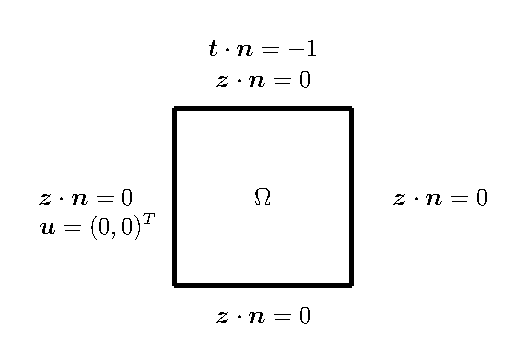
\includegraphics[width=0.5\textwidth]{canteliver_diag_crop.eps}}
  \subfloat[]{\label{fig:cantilever_plot}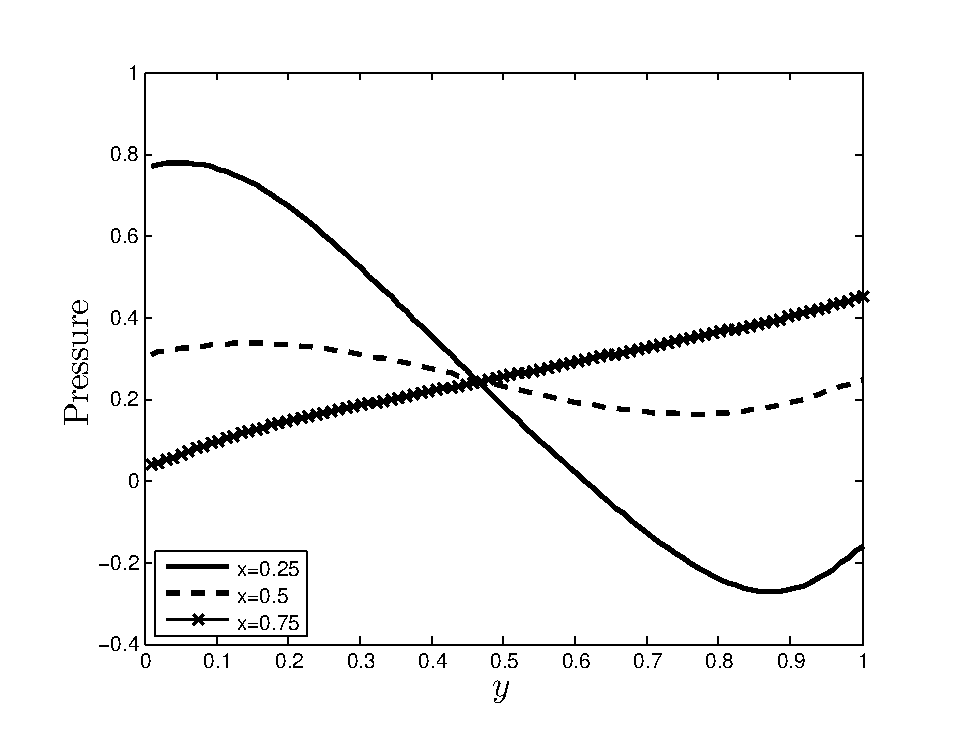
\includegraphics[width=0.5\textwidth]{cantilever_plot.eps}}
\caption{(a) Boundary conditions for the cantilever bracket problem. (b) Pressure solution of the cantilever bracket problem at $t=0.005$.}
\end{figure}

%%%%%%%%%%%%%%%%%%%%%%%%%%%%%%%%%%%%%%%%%%%%%%%%%%%%%%%%%%%%%%%%%%%%%%%%%%%%%%%%%%%%%%%%%%%%%%%%%%%%
%     3D unconfined compression stress relaxation
%%%%%%%%%%%%%%%%%%%%%%%%%%%%%%%%%%%%%%%%%%%%%%%%%%%%%%%%%%%%%%%%%%%%%%%%%%%%%%%%%%%%%%%%%%%%%%%%%%%%

\subsection{3D unconfined compression stress relaxation}
\label{sec:unconfined}
In this test, a cylindrical specimen of porous tissue is exposed to a prescribed displacement in the axial direction while left free to expand radially. (Note that the two plates are not explicitly modelled in the simulation, but are realised through displacement boundary conditions.) After loading the tissue, the displacement is held constant while the tissue relaxes in the radial direction due to interstitial fluid flow through the radial boundary. For the special case of a cylindrical geometry \cite{armstrong1984analysis} found a closed-form analytical solution for the radial displacement $u$ given by
\begin{equation}
 \frac{u}{a}(a,t)=\epsilon_{0}\left[ \nu + (1-2\nu)(1-\nu) \sum^{\infty}_{n=1}\frac{\exp{( -\alpha_n^{2} \frac{M \perm t}{a^{2}}}) }{ \alpha_{n}^{2}(1-\nu)^{2}-(1-\nu) }  \right].
\end{equation}
where $\alpha_n$ are the solutions to the characteristic equation $J_{1}(x)-(1-\nu)xJ_{0}(x)/(1-2\nu)=0,$ where $J_{0}$ and $J_{1}$ are Bessel functions, $\epsilon_{0}$ is the amplitude of the applied axial strain, $a$ is the radius of the cylinder, and $t_{g}$ is the characteristic time of diffusion (relaxation) $t_{g}= a^{2}/M k$, where $M=\lambda + 2\mu$ is the P-wave modulus of the elastic solid skeleton, and $\perm$ is the permeability.


%We computed the solution to $T=10\mbox{s}$  using a time step $\Delta t=0.1\mbox{s}$ and the radial displacement predicted by our implementation (Figure \ref{fig:anal_unconfined_plot}) using a value of $\delta=0.001$ gives a root mean squared error of $6.7\times 10^{-4}$ against the analytical solution provided by \cite{armstrong1984analysis}, and yields a stable solution. The same test problem has also been used to verify other poroelastic software such as FEBio \cite{maas2012febio}.
The analytical solution available for this test problem describes the displacement of the outer radius which is directly dependent on the amount of mass in the system since the porous medium is assumed to be incompressible and fully saturated. It is therefore an ideal test problem for analyzing the effect that the added stabilization term has on the conservation of mass. In Figure \ref{fig:anal_unconfined_plot} we can see that for large values of $\delta$ the numerical solution loses mass faster and comes to a steady state that has less mass than the analytical solution. This is a clear limitation of the method and the stability parameter therefore needs to be chosen carefully. However, for 3D problems $\delta$ can be chosen to be very small so this effect is negligible, as can be seen in Figure \ref{fig:anal_unconfined_plot} for a stable value of $\delta=0.001$.

\begin{figure}[h]
  \centering
  \subfloat[]{\label{fig:unconfined_diag}\includegraphics[width=0.4\textwidth]{unconfined_diag.eps}}
  \subfloat[]{\label{fig:unconfined_sim}\includegraphics[width=0.5\textwidth]{unconfined.eps}}
  \label{fig:animals}
\caption{ (a) Sketch of the test problem. The porous medium is being compressed between two smooth impervious plates. The frictionless plates permit the porous medium to expand in order to conserve volume and then to gradually relax as the fluid seeps out radially. (b) Pressure field solution at $t=5$, using a mesh with 28160 tetrahedra.}
\end{figure}
 \begin{figure}[h]
\begin{center}
\includegraphics[width=0.45\linewidth]{unconfined_results_delta.eps}
\caption{Normalized radial displacement versus normalized time calculated using the analytical
solution, and using the proposed numerical method with different values of $\delta$. At $t=0$ the radial expansion is half of the axial compression indicating the instantaneous incompressibility of the poroelastic tissue. The final amount of tissue recoil depends on the intrinsic Poisson ratio of the tissue skeleton.}
\label{fig:anal_unconfined_plot}
\end{center}
\end{figure}
